\documentclass[a4paper,12pt]{article}
\usepackage{amsmath,amsfonts,amsthm}
\usepackage[latin1]{inputenc}
\usepackage[T1]{fontenc}
\usepackage[spanish]{babel}
\usepackage{graphicx}
\parskip=2mm
\topmargin=-1cm
\oddsidemargin=0cm
\textwidth=16cm
\textheight=21cm
\parindent=1,5cm
\pagestyle{empty}
\newcommand{\horrule}[1]{\rule{\linewidth}{#1}} % Create horizontal rule command with 1 argument of height

\title{	
\normalfont \normalsize 
\textsc{Universidad de La Habana, Facultad de Matem\'{a}tica y Computaci\'{o}n } \\
Departamento de Inteligencia Artificial\\[25pt] % Your university, school and/or department name(s)
\horrule{0.5pt} \\[0.4cm] % Thin top horizontal rule
\huge Desarrollo de un modelo para la predicci\'{o}n de los Juegos Panamericanos de Lima 2019 utilizando Machine Learning \\ % The assignment title
\horrule{2pt} \\[0.5cm] % Thick bottom horizontal rule
}
\author{\\\name Ana Paula Arg\"{u}elles Terr\'{o}n C-111
\\
\name Mauro J. Bolado Vizoso C-111
\\ 
\name Daniel Alejandro C\'{a}rdenas Cabrera C-113 
\\
\name Javier Alejandro Oramas L\'{o}pez C-121}

\date{16 de Julio de 2019} % Today's date or a custom date
\begin{document}
\maketitle
\newpage
\section{Introducci\'{o}n}
	\cline{-}El presente art\'{i}culo aborda el tema de realizar una predicci\'{o}n a partir de un m\'{e}todo de Machine Learning para obtener un pron\'{o}stico aproximado con vista a los Juegos Panamericanos que tendr\'{a}n lugar en Lima este 2019.
 	\cline{-} Para ello se presentar\'{a} a continuaci\'{o}n conceptos introductorios al tema sin los cuales fuese imposible el total entendimiento de lo desarrollado.
	\cline{-} Inteligencia:Facultad intelectual con que se captan y forman ideas y se crean  relaciones. 
	\cline{-} Aprendizaje: Aprendizaje es un cambio en la disposici\'{o}n o capacidad humana, que persiste durante un tiempo y no pueden atribuirse simplemente a los procesos de crecimiento biol\'{o}gico.(Gag\~{n}\'{e}, 1987).
	\cline{-} Inteligencia Artificial: La Inteligencia Artificial es la ciencia cibern\'{e}tica que se encarga de la elaboraci\'{o}n de sistemas que "le den una soluci\'{o}n inteligente a los problemas", dicho de otra manera los sistemas inteligentes solucionan problemas que de ser resueltos por un humano requrir\'{i}an un comportamiento inteligente. La Inteligencia Artificial, con todas sus tendencias, es una de las disciplinas m\'{a}s prometedoras de las ciencias de la computaci\'{o}n y a la que varios cientif\'{i}cos est\'{a}n dedicando ingentes esfuerzos en todo el mundo.
	\cline{-} Los cient\'{i}ficos que han abordado y abordan este campo se encuentran con los problemas que ello conlleva:
	\begin{enumerate}
	\item -	Los computadores no pueden manejar (no contienen) verdaderos significados.
	\item -	Los computadores no tienen autoconciencia (emociones, sociabilidad, etc.). 
	\item -	Un computador solo puede hacer aquello para lo que est\'{a} programado.
	\item -	Las m\'{a}quinas no pueden pensar realmente. 
	\end{enumerate}
Problemas a los cuales tambi\'{e}n se enfrenta este trabajo.
\newpage
\section{Desarrollo}
\cline{-} Ante todo se procedi\'{o} a la recopilaci\'{o}n de los datos necesarios para el aprendizaje del programa, de acuerdo a los objetivos requeridos. Estos son esenciales para cualquier trabajo con Machine Learning o Artificial Intelligence (A.I.) por sus siglas en ingl\'{e}s, ya que sin una buena selecci\'{o}n y manejo de los datos no se puede llegar a resultados fiables.
\cline{-} Una vez obtenidos los datos a procesar se impuso la necesidad de establecer el algoritmo a utilizar para su procesamiento.
\cline{-} Cuando se pretende predecir un resultado, las personas con conocimentos del tema, sin dudas, en primera instancia piensan en utilizar un algoritmo b\'{a}sico, "Lineal Regression", que aproxima el resultado trazando la recta que mejor describa el comportamiento de los mismos, aportando una soluci\'{o}n al problema. No obstante, el resultado obtenido por este m\'{e}todo, en algunos casos, como en el nuestro, es bastante impreciso dado que la gr\'{a}fica producida por los datos no describe una funci\'{o}n lineal, en discordancia con el algoritmo antes mencionado. Por ello en nuestro caso optamos por implementar un algoritmo utilizando "Polynomial Regression". 
\cline{-} Para el desarrollo de dichos algoritmos se utilizaron las siguientes librerias de Python:
\begin{enumerate}
\item - pandas
\item - sklearn
\item - matplotlib
\item - numpy
\end{enumerate}
\cline{-} Pandas es la librer\'{i}a que permite importar los datos almacenados en un archivo cuya extensi\'{o}n sea .csv para su manejo desde el programa.
\cline{-} Sklearn contiene ya implementados los algoritmos de Machine Learning previamente mencionados y proporciona muchas facilidades con el manejo de datos para su procesamiento.
\cline{-} Matplotlib permite graficar los datos para una mejor visualizaci\'{o}n de estos.
\cline{-} Numpy permite convertir las listas de datos en array para un mejor manejo de estos.\begin{figure}[hbtp]
\caption{Primer fragmento del c\'{o}digo}
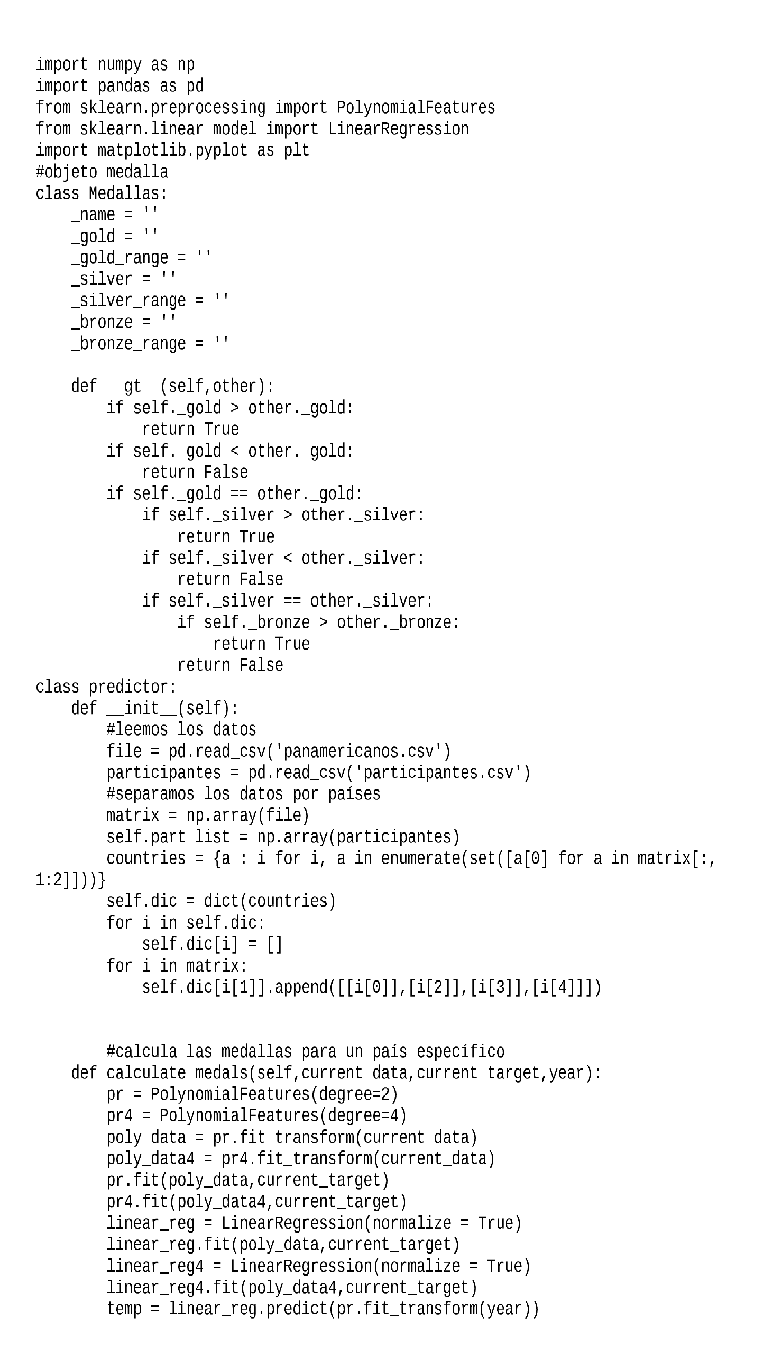
\includegraphics[scale=0.7]{first_part.png}
\end{figure}
\newpage
\cline{-} En este fragmento se puede apreciar como se importan las librer\'{i}as anteriormente mencionadas, seguido de la implementaci\'{o}n de la clase medalla para su posterior uso en el programa y se da paso a la implementaci\'{o}n del algoritmo que resuelve nuestro problema.
\begin{figure}[hbtp]
\caption{Segundo fragmento del c\'{o}digo}
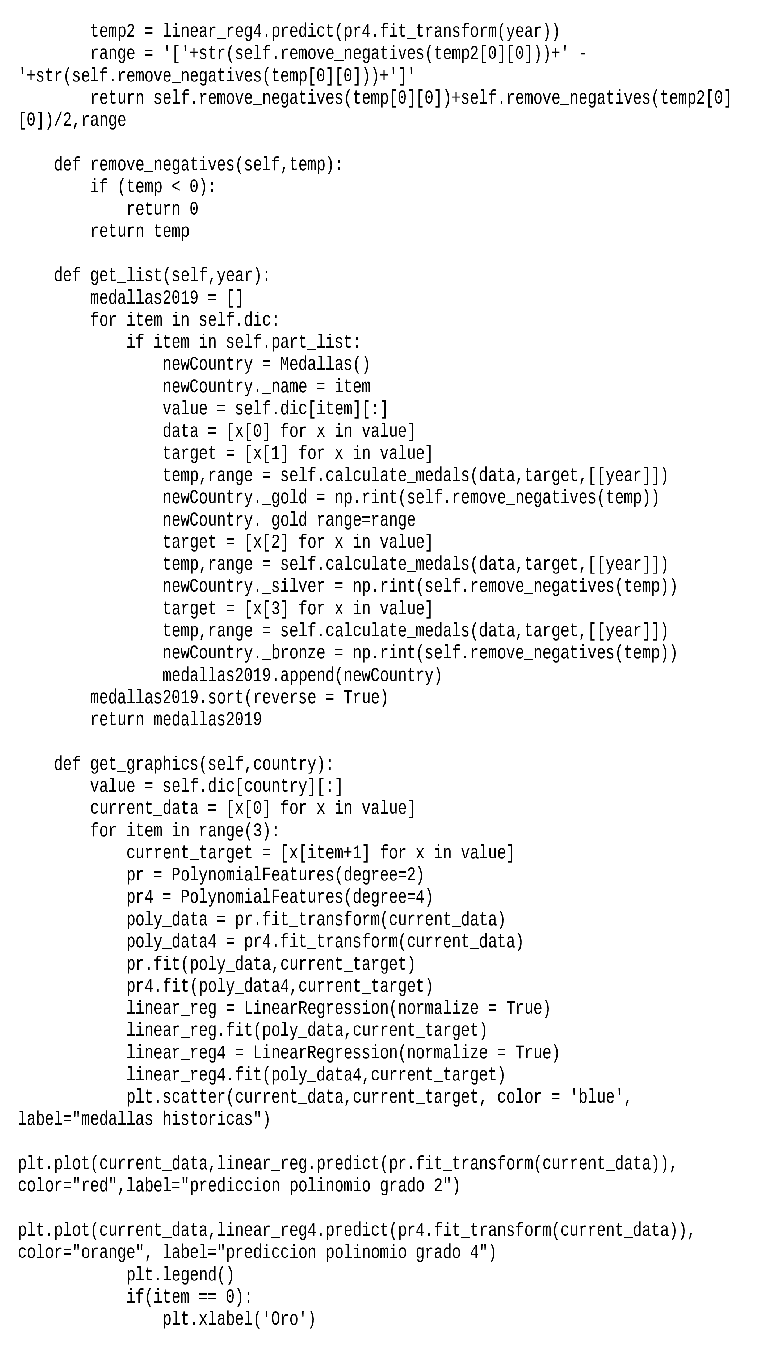
\includegraphics[scale=0.7]{second_part.png}
\end{figure}
\newpage
\begin{figure}[hbtp]
\caption{Continuaci\'{o}n del segundo fragmento}
\centering
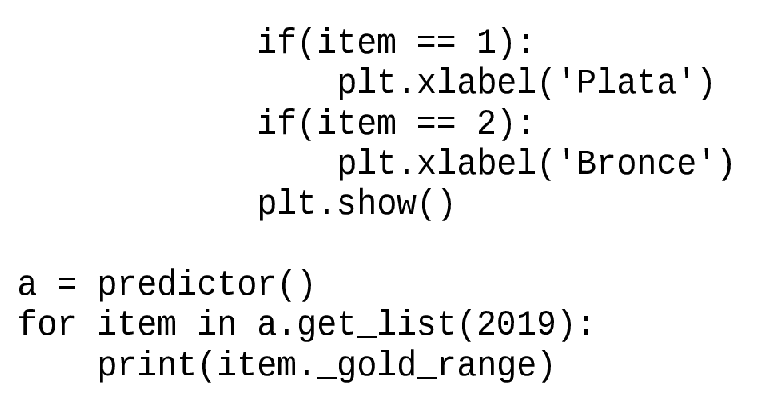
\includegraphics[scale=0.4]{third.png}
\end{figure}
\cline{-} Con el c\'{o}digo anterior dado los diferentes grados del polinomio se obtienen como resultados las siguientes tablas:
\begin{figure}[hbtp]
\caption{Resultado obtenido con el polinomio de grado 2}
\centering
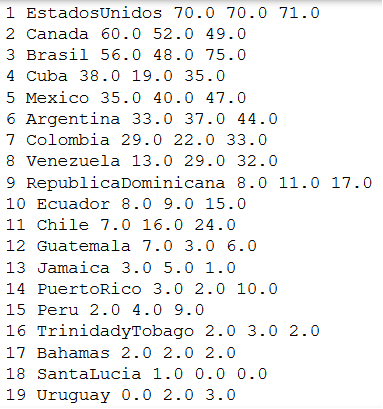
\includegraphics[scale=1]{19_primeros_polinomio_grado_2.png}
\end{figure}
\begin{figure}[hbtp]
\caption{Resultado obtenido con el polinomio de grado 4}
\centering
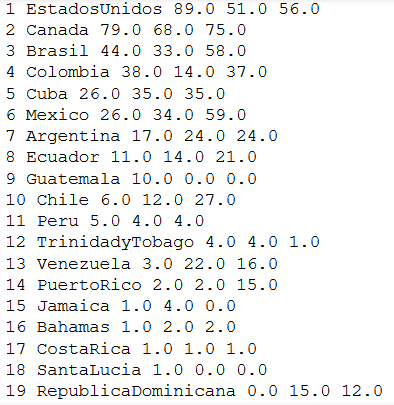
\includegraphics[scale=1]{19_primeros_polinomio_grado_4.png}
\end{figure}
\begin{figure}[hbtp]
\caption{Resultado final producto de la uni\'{o}n de las predicciones anteriores}
\centering
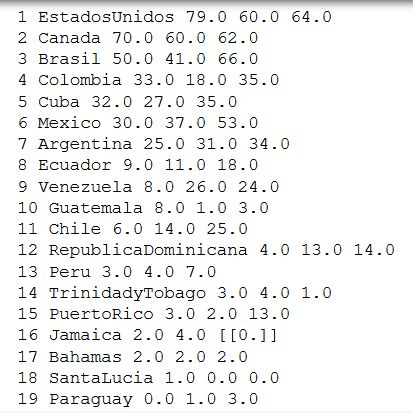
\includegraphics[scale=1]{19_primeros_prediccion_combinada.png}
\end{figure}

\newpage
\section{Conclusiones}
\cline{-} Como se pudo apreciar los resultados obtenidos por el programa se asemejan a la actuaci\'{o}n real de cada uno de los pa\'{i}ses a los largo de la historia, salvo en excepciones donde se rompieron los pron\'{o}sticos, se\~{n}al de un buen funcionamiento y la aceptabiladad del pron\'{o}stico obtenido.
\newpage
\section{Anexos}
\begin{figure}[hbtp]
\caption{Gr\'{a}fica hist\'{o}rica de los oro de Cuba}
\centering
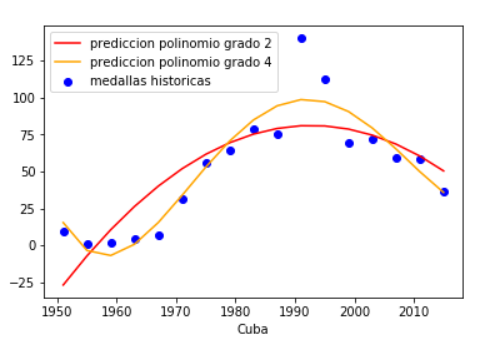
\includegraphics[scale=1]{cuba_oro.png}
\end{figure}
\begin{figure}[hbtp]
\caption{Gr\'{a}fica hist\'{o}rica de los bronce de Cuba}
\centering
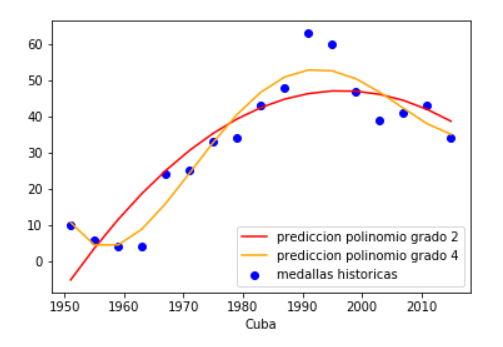
\includegraphics[scale=1]{cuba_bronce.png}
\end{figure}
\begin{figure}[hbtp]
\caption{Gr\'{a}fica hist\'{o}rica de las plata de Cuba}
\centering
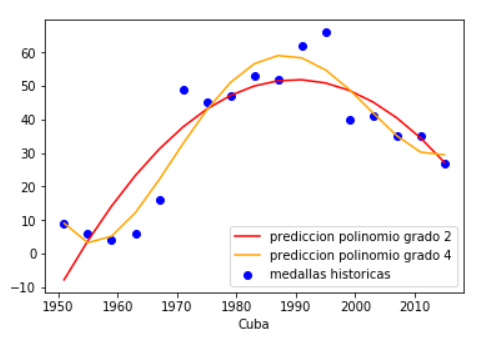
\includegraphics[scale=1]{cuba_plata.png}
\end{figure}

\end{document}
